% !TeX spellcheck = en-US
% !TeX encoding = utf8
% !TeX program = pdflatex
% !BIB program = biber
% -*- coding:utf-8 mod:LaTeX -*-


% vv  scroll down to line 200 for content  vv


\let\ifdeutsch\iffalse
\let\ifenglisch\iftrue
\input{pre-documentclass}
\documentclass[
  % fontsize=11pt is the standard
  a4paper,  % Standard format - only KOMAScript uses paper=a4 - https://tex.stackexchange.com/a/61044/9075
  twoside,  % we are optimizing for both screen and two-side printing. So the page numbers will jump, but the content is configured to stay in the middle (by using the geometry package)
  bibliography=totoc,
  %               idxtotoc,   %Index ins Inhaltsverzeichnis
  %               liststotoc, %List of X ins Inhaltsverzeichnis, mit liststotocnumbered werden die Abbildungsverzeichnisse nummeriert
  headsepline,
  cleardoublepage=empty,
  parskip=half,
  %               draft    % um zu sehen, wo noch nachgebessert werden muss - wichtig, da Bindungskorrektur mit drin
  draft=false
]{scrbook}
\input{config}


\usepackage[
  title={Visual Exploration Of Light Transport In Path Tracing},
  author={Giulio Martella},
  type=master,
  institute=vis, % or other institute names - or just a plain string using {Demo\\Demo...}
  course={Computer Science},
  examiner={Jun.-Prof. Dr.\ Michael Sedlmair},
  supervisor={Dr.\ Guido Reina\\Michael Becher,\ M.Sc.\\Patrik Gralka,\ M.Sc.},
  startdate={July 1, 2020},
  enddate={January 4, 2021}
]{scientific-thesis-cover}

\input{acronyms}

\makeindex

\usepackage{subcaption}
\usepackage{sidecap}
\usetikzlibrary{patterns}

\begin{document}

%tex4ht-Konvertierung verschönern
\iftex4ht
  % tell tex4ht to create picures also for formulas starting with '$'
  % WARNING: a tex4ht run now takes forever!
  \Configure{$}{\PicMath}{\EndPicMath}{}
  %$ % <- syntax highlighting fix for emacs
  \Css{body {text-align:justify;}}

  %conversion of .pdf to .png
  \Configure{graphics*}
  {pdf}
  {\Needs{"convert \csname Gin@base\endcsname.pdf
      \csname Gin@base\endcsname.png"}%
    \Picture[pict]{\csname Gin@base\endcsname.png}%
  }
\fi

%\VerbatimFootnotes %verbatim text in Fußnoten erlauben. Geht normalerweise nicht.

\input{commands}
\pagenumbering{arabic}
\Titelblatt

%Eigener Seitenstil fuer die Kurzfassung und das Inhaltsverzeichnis
\deftripstyle{preamble}{}{}{}{}{}{\pagemark}
%Doku zu deftripstyle: scrguide.pdf
\pagestyle{preamble}
\renewcommand*{\chapterpagestyle}{preamble}



%Kurzfassung / abstract
%auch im Stil vom Inhaltsverzeichnis
\ifdeutsch
  \section*{Kurzfassung}
\else
  \section*{Abstract}
\fi

<Short summary of the thesis>

\cleardoublepage


% BEGIN: Verzeichnisse

\iftex4ht
\else
  \microtypesetup{protrusion=false}
\fi

%%%
% Literaturverzeichnis ins TOC mit aufnehmen, aber nur wenn nichts anderes mehr hilft!
% \addcontentsline{toc}{chapter}{Literaturverzeichnis}
%
% oder zB
%\addcontentsline{toc}{section}{Abkürzungsverzeichnis}
%
%%%

%Produce table of contents
%
%In case you have trouble with headings reaching into the page numbers, enable the following three lines.
%Hint by http://golatex.de/inhaltsverzeichnis-schreibt-ueber-rand-t3106.html
%
%\makeatletter
%\renewcommand{\@pnumwidth}{2em}
%\makeatother
%
\tableofcontents

% Bei einem ungünstigen Seitenumbruch im Inhaltsverzeichnis, kann dieser mit
% \addtocontents{toc}{\protect\newpage}
% an der passenden Stelle im Fließtext erzwungen werden.

%\listoffigures
%\listoftables

%Wird nur bei Verwendung von der lstlisting-Umgebung mit dem "caption"-Parameter benoetigt
%\lstlistoflistings
%ansonsten:
%\ifdeutsch
%  \listof{Listing}{Verzeichnis der Listings}
%\else
%  \listof{Listing}{List of Listings}
%\fi

%mittels \newfloat wurde die Algorithmus-Gleitumgebung definiert.
%Mit folgendem Befehl werden alle floats dieses Typs ausgegeben
%\ifdeutsch
%  \listof{Algorithmus}{Verzeichnis der Algorithmen}
%\else
%  \listof{Algorithmus}{List of Algorithms}
%\fi
%\listofalgorithms %Ist nur für Algorithmen, die mittels \begin{algorithm} umschlossen werden, nötig

% Abkürzungsverzeichnis
%\printnoidxglossaries

\iftex4ht
\else
  %Optischen Randausgleich und Grauwertkorrektur wieder aktivieren
  \microtypesetup{protrusion=true}
\fi

% END: Verzeichnisse


% Headline and footline
\renewcommand*{\chapterpagestyle}{scrplain}
\pagestyle{scrheadings}
\pagestyle{scrheadings}
\ihead[]{}
\chead[]{}
\ohead[]{\headmark}
\cfoot[]{}
\ofoot[\usekomafont{pagenumber}\thepage]{\usekomafont{pagenumber}\thepage}
\ifoot[]{}


%%%%%%%%%%%%%%%%%%%%%%%%%%%%%%%%%%%%%%%%%%%%%%%%%%%%%%%%%%%%%%%%%%%%%%%%%%%%%%
%
% Main content starts here
%
%%%%%%%%%%%%%%%%%%%%%%%%%%%%%%%%%%%%%%%%%%%%%%%%%%%%%%%%%%%%%%%%%%%%%%%%%%%%%%


\chapter{Introduction}

\section{Motivation}
\label{motivation}
This project has been based upon the idea of giving the user the power to visually and interactively explore all the paths generated by a path tracer during rendering. In the very first vision, a user should have been able to select a portion of a surface of the 3d scene the tracer has been run upon and see the paths that bounce there with a bunch of useful data. To be able to do that the whole set of paths shoot by a tracer are needed: by the very stochastic nature of a path tracer, it is impossible to determine which paths will end up bouncing where without resolving them all first. That is why it has been decided it was essential to store data about each path during the rendering process. To make the tool usable in most possible use cases, it had to be able to plug into an existing path tracer and this lead to the conception of the tool as a two software pieces suite: a \textit{data gatherer library} called \texttt{gatherer} and a \textit{visualization client} called \texttt{gathererclient}.

%Now this “useful data” was not extremely well-defined during those early stages, so most of the efforts have been directed to the very essential: rendering the requested paths keeping interactivity.

\section{Technology}
\label{technology}

The data gatherer has been developed as a header-only C++17\footnote{C++17 is the informal name of the ISO/IEC 14882:2017 standard. \url{https://www.iso.org/standard/68564.html}} library. The choice was motivated by the belief --- not backed by any data --- that most path tracers, included the ones written by students, are written in C++. In hindsight, probably writing it in pure C would have made it potentially compatible with more path tracers; after all it uses very few features of C++. 

Deciding the technologies to use for the visualization client took more careful thinking, since it was clear it would be the biggest software piece in the context of this project. The final combination consists in:
\begin{description}
	\item[C++] Due to the available expertise, the other plausible languages were Python and --- for a very brief moment --- Julia, but they were discarded due to the necessity of managing memory and threads directly. C has been considered too, but STL and OOP made the scale tip over C++. As for the data gatherer, C++17 is used.
	\item[“Raw” OpenGL] Rendering hundreds of thousands paths in an interactive and fully customizable fashion was perceived since the beginning as no easy task and it made clear the necessity to be able to control and program every possible stage of the rendering pipeline. Due to this, visualization frameworks such as VTK \cite{vtk2006} had been ruled out immediately in favor of just GLEW and GLFW3 to provide an OpenGL 4.6 Core Profile context.
	\item[Dear ImGui] Since all rendering customization needs came from the interactive 3d rendering of paths and scenes, using just OpenGL to build a GUI from scratch would have been insane and so a GUI framework had to be chosen. The final candidates were Qt5 and Dear ImGui\footnote{\url{https://github.com/ocornut/imgui}} but since ImGui was not completely familiar to the author, it has been chosen due to educational purposes.
	\item[Boost Log and Filesystem] It seemed like a good idea to have a complete logger and a filesystem library with a STL-like style and it led to the adoption of the Boost Log\footnote{\url{https://www.boost.org/doc/libs/1_75_0/libs/log/doc/html/index.html}} and Boost Filesystem\footnote{\url{https://www.boost.org/doc/libs/1_39_0/libs/filesystem/doc/index.htm}} libraries. Since it is not a crucial dependency, it might be removed in a future development.
\end{description}

Both the gatherer and the visualization client use a header-only math library called \textit{math.hpp}\footnote{\url{https://github.com/giuliom95/math}} to handle vector and matrix types and operations. It includes the \textit{half} library\footnote{\url{http://half.sourceforge.net/}} which is an implementation of the 16 bits floating point number representation, commonly called half precision float or just \texttt{half}, as described by the IEEE 754 standard\footnote{\url{https://ieeexplore.ieee.org/document/8766229}}.

\section{Background}

To fully comprehend the topics and challenges presented in this work a background is needed.

\subsection{The rendering equation}
\textit{Photorealistic rendering} is the process that given a mathematical description of a 3-dimensional scene outputs an as life-like as possible image, know as \textit{render}. The process simulates how light travels from light sources to a --- abstract --- camera sensor while interacting with the scene.
\chapter{The tool}

\section{General description}
\label{tool_general_description}
The tool has two components: a \textit{data gatherer} and a \textit{visualization client}.

The data gatherer is a C++ header-only class of which methods have to be called within the main loop of any unidirectional path tracer. It stores to disk data generated --- and usually discarded --- by the path tracer during rendering. For each path shoot by the renderer the tool stores its transported radiance, its camera sample, and the world positions of its bounces. 

Once the rendering is done and the data is collected, the visualization client can be used to explore the gathered information. To allow interactive 3D exploration it also needs a scene description; this is not generated by the gatherer and it has to be provided separately by the user. The scene format used is novel, based on triangle meshes and it shares many similarities with glTF \cite{robinet2014gltf}. This peculiar choice has been done mainly to not do any assumptions on the kind of geometry representation the path tracer uses. In this way even path tracers that use exotic geometries can be analyzed with the tool --- at least until the user is able to convert whatever they are using in triangles.


\section{Data gatherer}

\subsection{The data to gather}
Until now, it has been said that the gatherer has to be able to store “the paths with some useful data”, but how does one store a path and what is useful data have not been defined yet. In the beginning, the focus was on just visualizing paths in an interactive scene rendering so that the user could see how paths interact with the scene. To achieve that it was clear the actual geometry of all paths had to be stored. This meant storing for each path a camera sample and all of its bounces.
Several ways of storing path bounces had been considered, such as storing each bounce as a direction and a distance, but the most naïve solution has been opted: each bounce is stored as a 3-dimensional point in world space.

This immediately raised some concerns about how much memory would be required to store all these points: let us calculate how many bytes it would take to just store the bounces of all paths needed to produce image \ref{hall_render}. It is 512 pixels wide and 512 pixels tall, it has been rendered with 512 samples per pixel --- spp --- each with a depth of maximum 10 --- this means that each of the 512 paths shoot every pixel bounced in the scene at most 10 times. Storing the points as a triplet of single precision float numbers --- 4 bytes, the C++ built-in \texttt{float} type ---  we would have:
\begin{equation}
	\label{rough_bounce_size_estimation}
	(512 \times 512) pixels \times 512 spp \times 10 bounces \times 3 dimensions \times 4 bytes \approx 15GB
\end{equation}
\begin{figure}
	\centering
	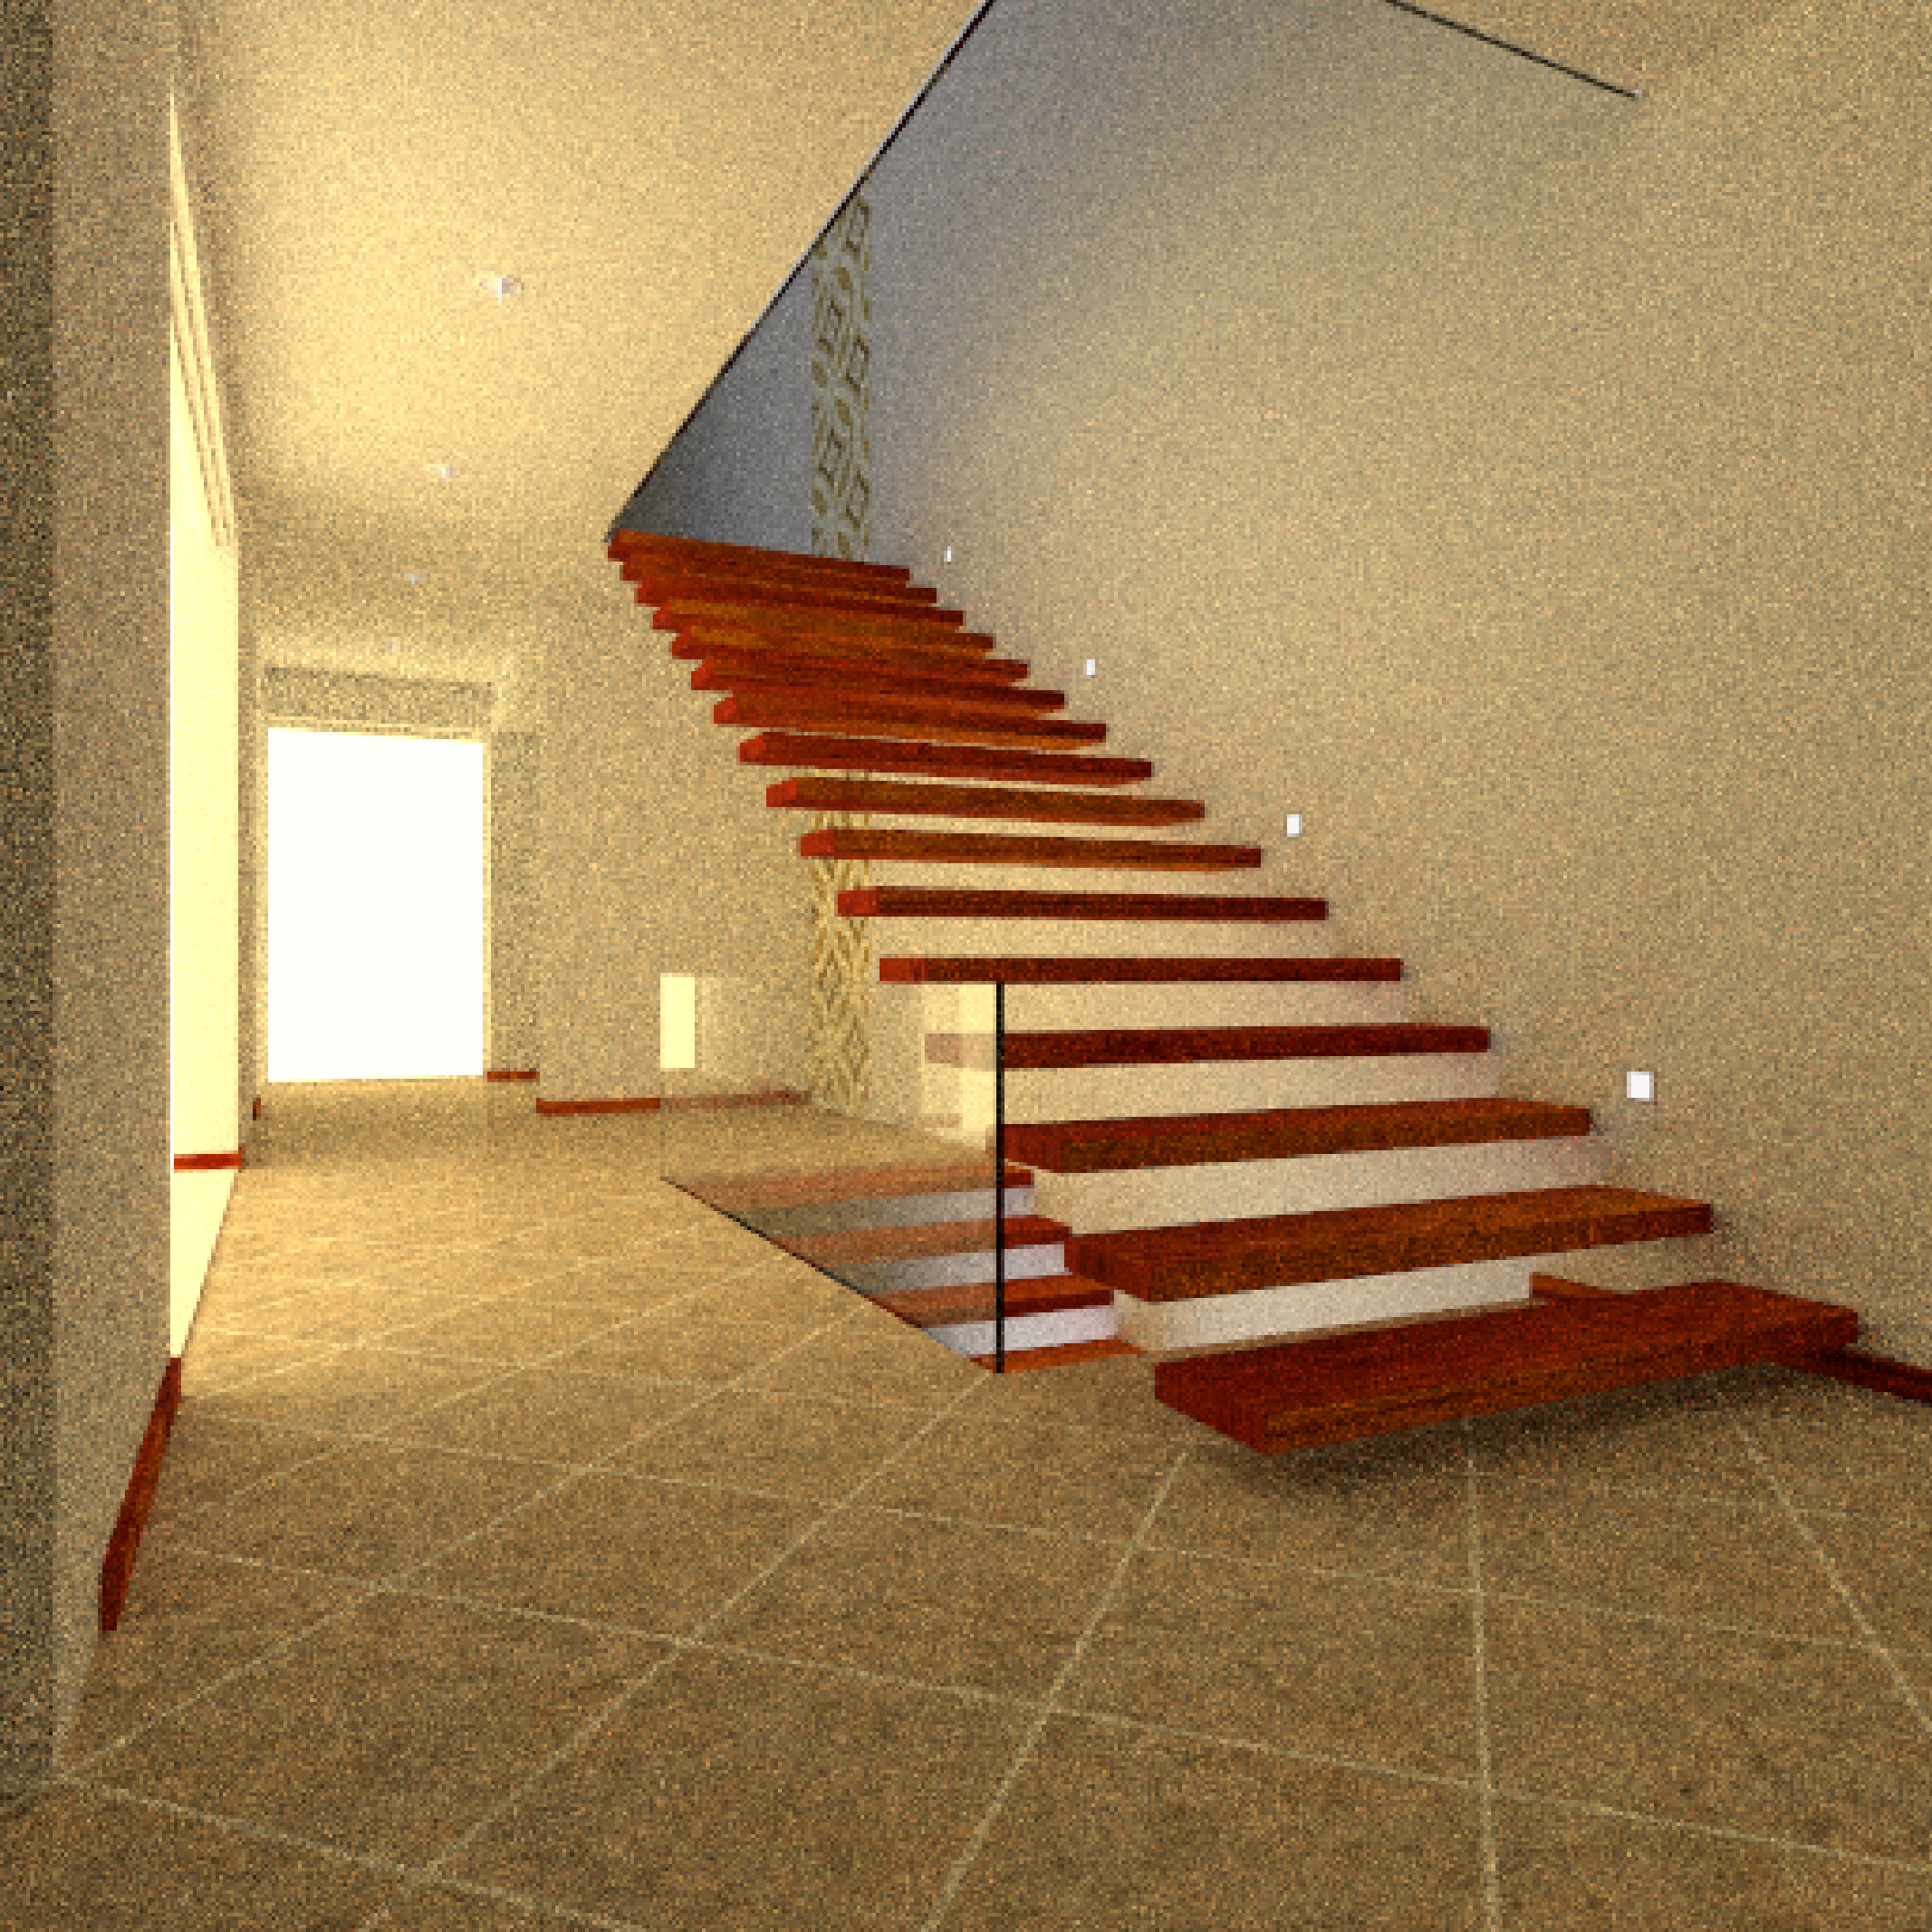
\includegraphics[height=8cm]{chapters/chapter_thetool/hall}
	\caption{\textit{Modern Hall} scene \cite{bitterliscenes} rendered by Yocto/GL \cite{pellacini2019yocto}. It is a 512x512, 512spp image; maximum bounces per path are set to 10.}
	\label{hall_render}
\end{figure}
As said just above, the paths in this case bounce at most 10 times: most paths are terminated way before either when they bounce out of the scene or --- in some path tracers --- they hit a light. This leads to the need of an additional buffer storing the amount of bounces each path has. Put with computer graphics terminology we might say the points positions buffer represents the \textit{geometry} of the paths while this “path lengths” buffer is the \textit{topology}. 
This new buffer needs to contain integers and, considering that the standard C++ \texttt{int} built-in type on x86\_64 machines is 4 bytes long, we would have that the size of the buffer in the context of figure \ref{hall_render} would approximately be:
\begin{equation}
	\label{rough_lenghts_size_estimation}
	(512 \times 512) pixels \times 512 spp \times 4 bytes \approx 500MB
\end{equation}
Now this is not an unmanageable amount of data, but since the tool has to be usable on consumer grade machines, reducing those number has been one of the main priorities during the early stages of development. The most effective change that has been made is to simply use smaller primitive data types. 
Single precision floats had been almost immediately replaced with half-precision floating point numbers, effectively halving the size of the world positions buffers. Using the same assumptions made for equation \ref{rough_bounce_size_estimation}, we would have 7.5GB instead of 15GB.
Halving precision, beside a memory footprint reduction, comes with a reduction of actual precision and potential noticeable rounding errors; but since these numbers will mostly be directly used for visualization purposes with very little preprocessing, precision errors should not negatively impact the user experience.
Considering now the paths lengths buffer, in most reasonable cases, 1 byte per path would suffice: 255 bounces are more than enough for most cases. Examining equation \ref{rough_lenghts_size_estimation}, after the reduction from 4 bytes to 1 that buffer occupies approximately 128MB. Similar reasoning has been applied to all other buffers: every floating point number is half precision and every integer is made as small as reasonable.

To complete the spatial representation of the paths, an origin point, which is semantically not a bounce, was needed. For the sake of simplicity, an additional fake bounce lying on the render camera eye was added to each path. Due to its wasteful nature --- it adds 6 bytes per path which would accumulate to $512\times 512\times 512\times 6\approx 750MB$ in the case of figure \ref{hall_render} ---, this solution was hastily set aside; in the final version of the tool, the origin point of the paths is not stored in the dataset all together. The camera eye point that comes with the scene description --- see subsection \ref{scene_format} --- is implicitly considered the origin of all paths.

To fuel some components of the visualization client that have been developed over time, two other buffers are built by \texttt{gatherer}. One contains the camera samples and the other the radiance carried by each path. A camera sample is the correct position of a path on the virtual image sensor. The radiance of each path is just stored as a triplet of floats indicating the radiance carried by a path for the red, green and blue color components.

Focusing on implementation details it is clear that four binary data buffers have to be stored on disk. They could all be cramped into a single file but to make the loading code simpler, it has been decided to store each buffer in its own separate file.
This means that a full dataset has to be contained into a folder rather than a file. The folder, usually, but not necessarily, called \texttt{renderdata} contains two subfolders, \texttt{bounces} and \texttt{paths}.
This was made to logically separate buffers that contains data proper to entire paths --- like the lengths and the radiances --- to the ones relative to bounces --- the bounces positions. It may seem a little overzealous but it was made to support an easy and organized implementation of new buffers.

At the end of the day, there are 4 binary files and each contain:
\begin{description}
	\item[\texttt{bounces/positions.bin}] The world positions of all bounces of each path, stored as triplets of \texttt{half}.
	\item[\texttt{paths/lengths.bin}] The number of bounces of each path --- almost always called \textit{path length} in the code ---, each stored as a single \texttt{uint8\_t}.
	\item[\texttt{paths/radiance.bin}] The radiance carried by each path, stored as triplets of \texttt{half}.
	\item[\texttt{paths/camerasamples.bin}] The sample position on the film plane of each path. Each sample is stored in a \texttt{CameraSample} data structure\footnote{See listing \ref{gatherer_datastructures} for the actual C++ definition.}, which contains:
	\begin{itemize}
		\item A couple of \texttt{uint16\_t} indicating which pixel of the render image the sample belongs to.
		\item A couple of \texttt{half} $\in [0, 1]$ representing the position of the sample relative to the pixel, where $(0,0)$ is the upper left corner of the pixel and $(1,1)$ is the lower right one.
	\end{itemize} 
\end{description}

%TODO: maybe add an explanation on how is easy to understand which data is relative to which path?

\subsection{\texttt{Gatherer} class}
All data gathering is managed by a header-only library that exposes one single class called \texttt{Gatherer}. To correctly gather data from a path tracer the user must initialize an instance of \texttt{Gatherer} at any point before the main loop and then call its methods where appropriate while tracing paths. Signatures of the constructor and the methods of \texttt{Gatherer} is presented in Listing \ref{gatherer_signatures}.
The constructor needs a folder path where the data will be stored and the number of threads --- \texttt{nthreads} --- the path tracer will run on. The \texttt{addbounce} method has to be called every time a path bounces and the position of the bounce is final. It has that position in world coordinates as an argument  alongside a \textit{thread id}, an integer that goes from zero to \texttt{nthreads} and unequivocally identifies a thread.
When all the computations on a path are done and the radiance carried by it is known, the user has to call the \texttt{finalizepath} method passing the thread id, the radiance and a \texttt{CameraSample} struct --- see Listing \ref{gatherer_datastructures} for its layout.

As hinted by the \texttt{nthreads} and \texttt{tid} arguments of \texttt{Gatherer} methods, the class has been designed to be able to gather data from path tracers that evaluate paths on multiple threads parallelly. This extra effort has been made to not force users to use only single-threaded path tracers. It has to be though noted that the \texttt{Gatherer} class assumes each path is entirely resolved on just one thread: splitting the computations of a single path on multiple threads is not currently supported.

Datasets gathered from the rendering of high quality scenes can get big fast. To avoid any memory saturation problems and to leave as many resources as possible to the path tracing computations, \texttt{Gatherer} allocates a fixed amount of memory per thread and will use only that; it will store data on disk when any of these memory chunks are about to fill completely. In order to write to disk without introducing any software barrier in the multi thread code, each thread writes on a set of files that are written only it. The destructor of \texttt{Gatherer} takes care of stitching all these file sets into one, being extra careful to keep the indices consistent. This is sadly a fully disk-bound operation and it may take a while, especially on rather big dataset.


\begin{Listing}
	\begin{lstlisting}
class Gatherer
{
public:
	Gatherer
	(
		unsigned nthreads, 
		const std::filesystem::path& folder
	);

	void addbounce
	(
		unsigned tid, 
		Vec3h pos
	);

	void finalizepath
	(
		unsigned tid, 
		Vec3h radiance, 
		CameraSample sample
	);
}
	\end{lstlisting}
	\caption{Simplified \texttt{Gatherer} class definition with everything a user needs to gather data successfully.}
	\label{gatherer_signatures}
\end{Listing}

\begin{Listing}
	\begin{lstlisting}
using Vec3h = std::array<half, 3>;

class CameraSample
{
public:
	uint16_t i, j;
	half u, v;
};
	\end{lstlisting}
	\caption{Data structures used inside the \texttt{Gatherer} class. The \texttt{half} type contains a 16bit precision floating point number complying to the IEEE 754 standard.}
	\label{gatherer_datastructures}
\end{Listing}

%\begin{lstlisting}[caption={}, label=scene_json]
%\end{lstlisting}

\section{Visualization client}

\subsection{Path filters}
\begin{figure}
	\centering
	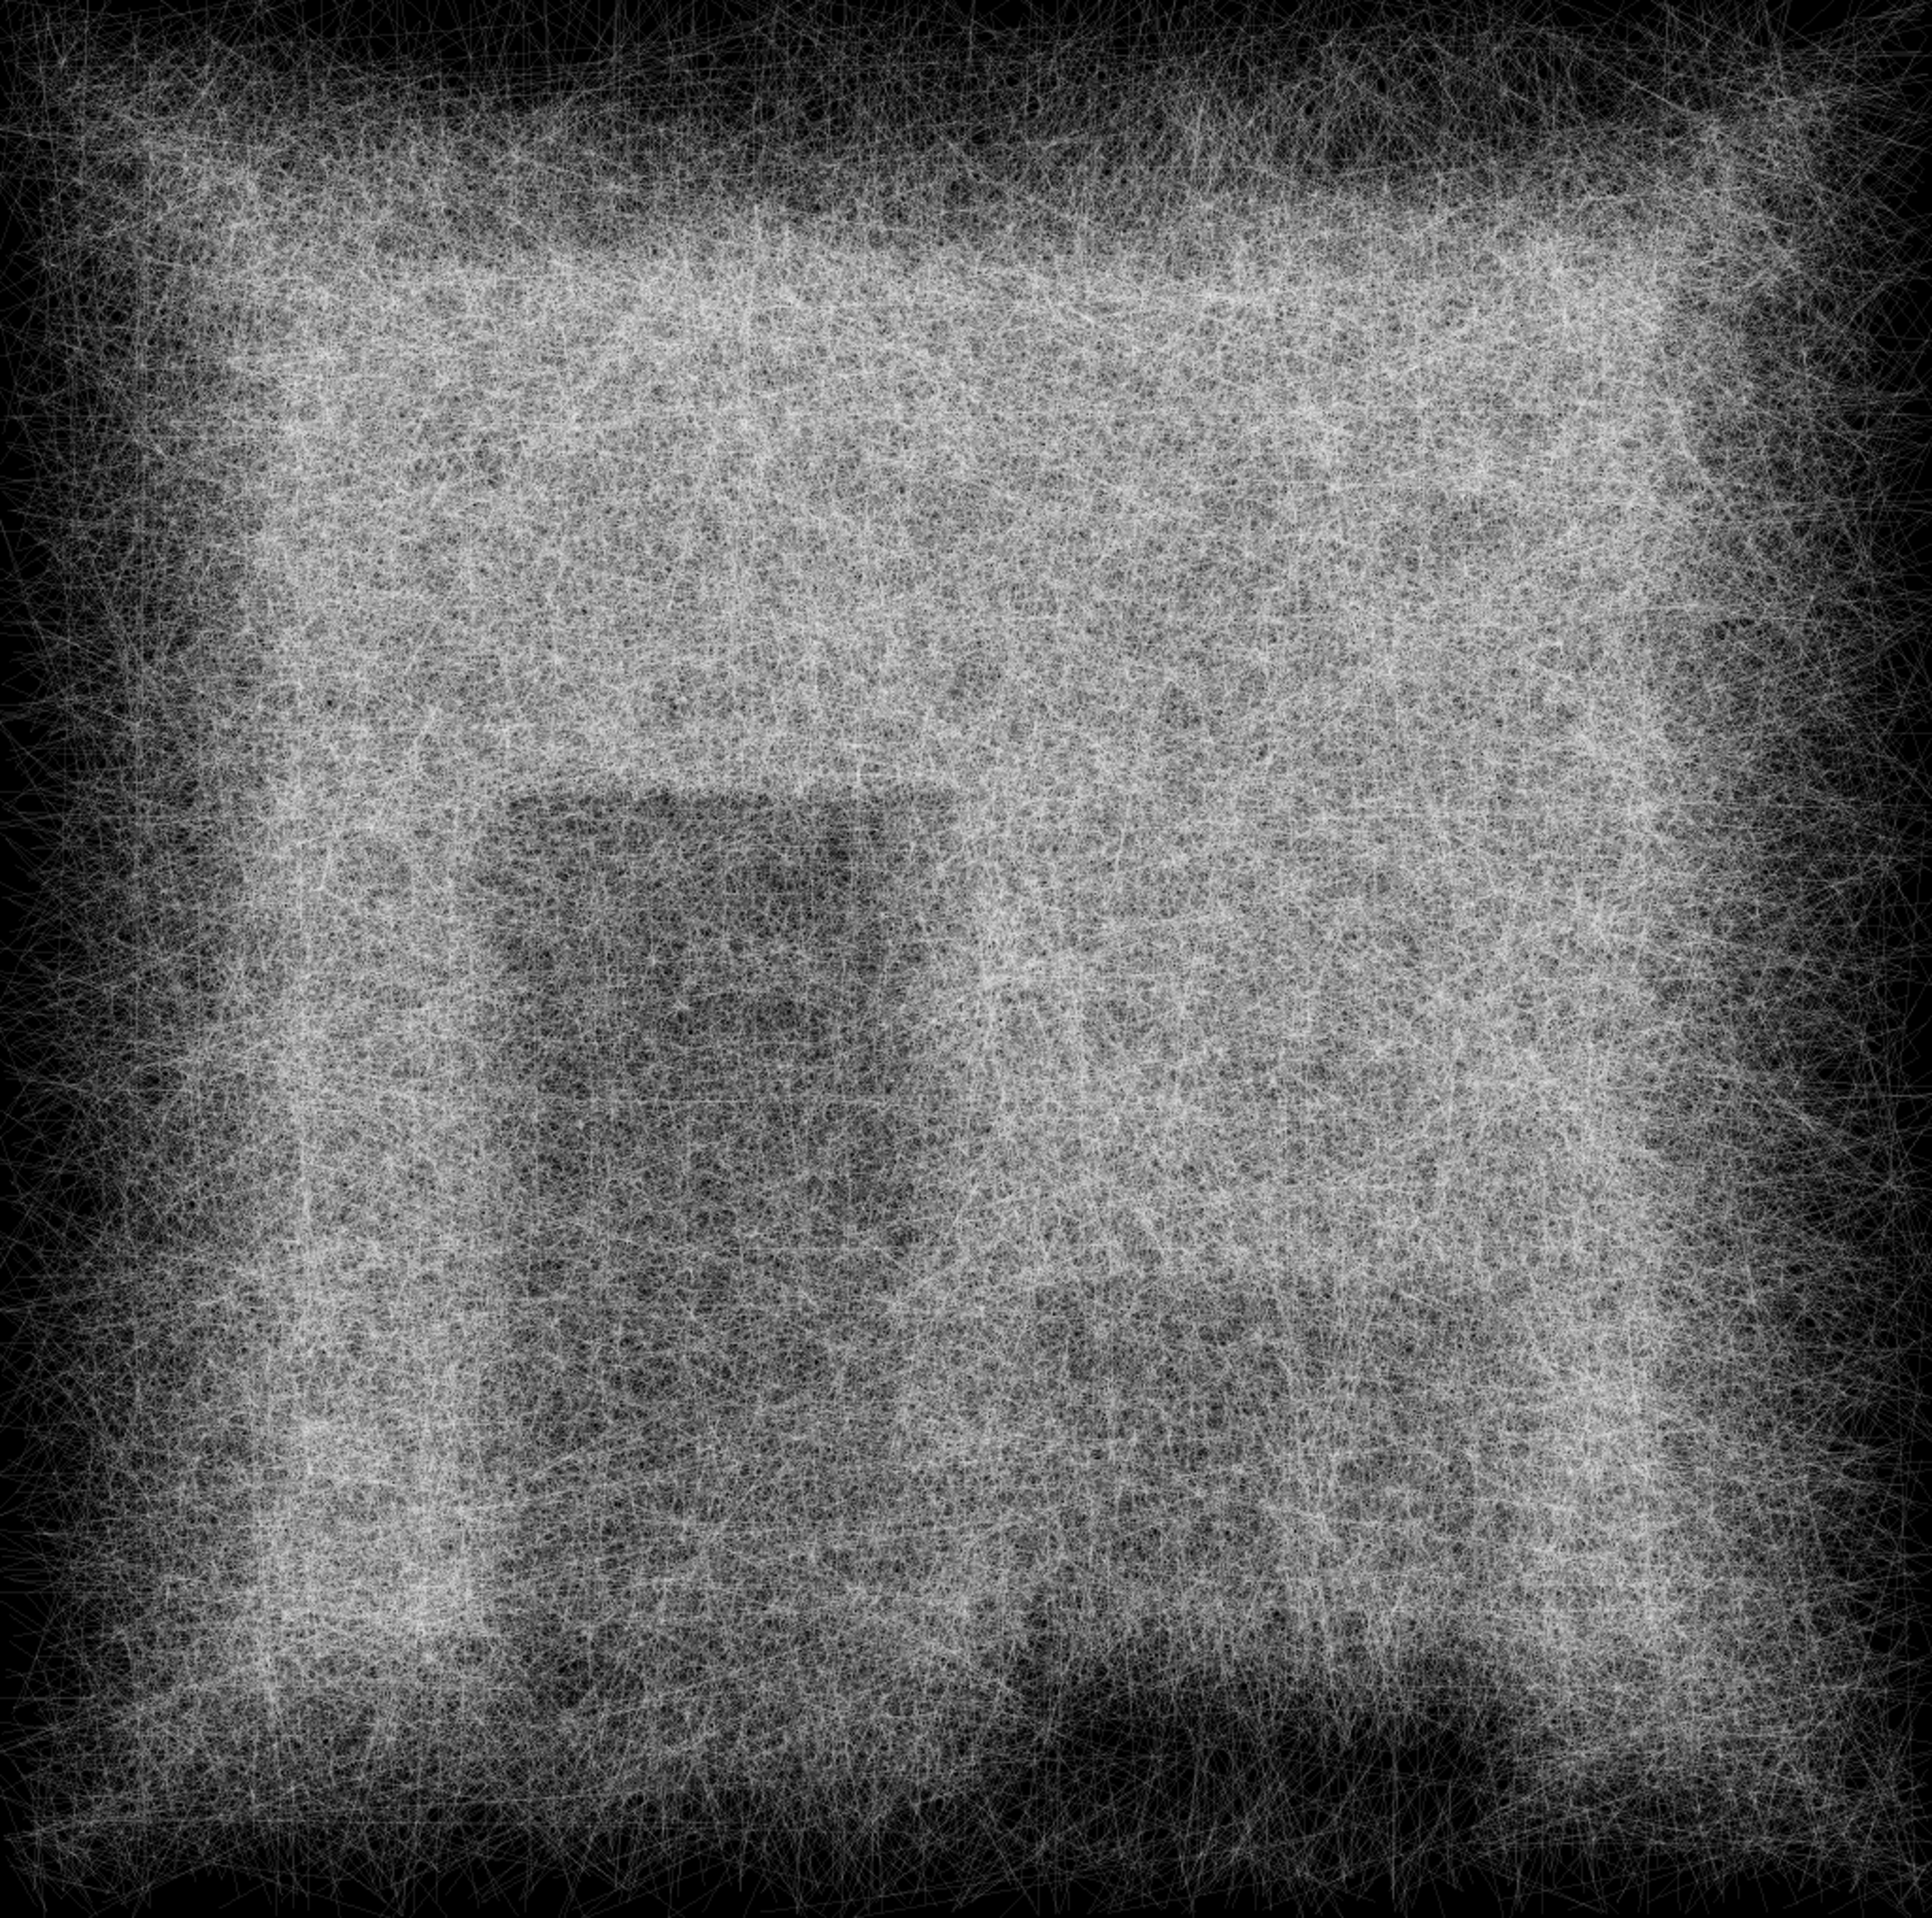
\includegraphics[height=8cm]{chapters/chapter_thetool/clutter_early.pdf}
	\caption{Visual clutter in an early render of all the paths used to path trace a $64 \times 64$, 1 spp image of the Cornell Box scene. The actual scene is not rendered to improve readability.}
	\label{visual_clutter}
\end{figure}

\begin{figure}
	\centering
	\begin{subfigure}[t]{0.49\linewidth}
		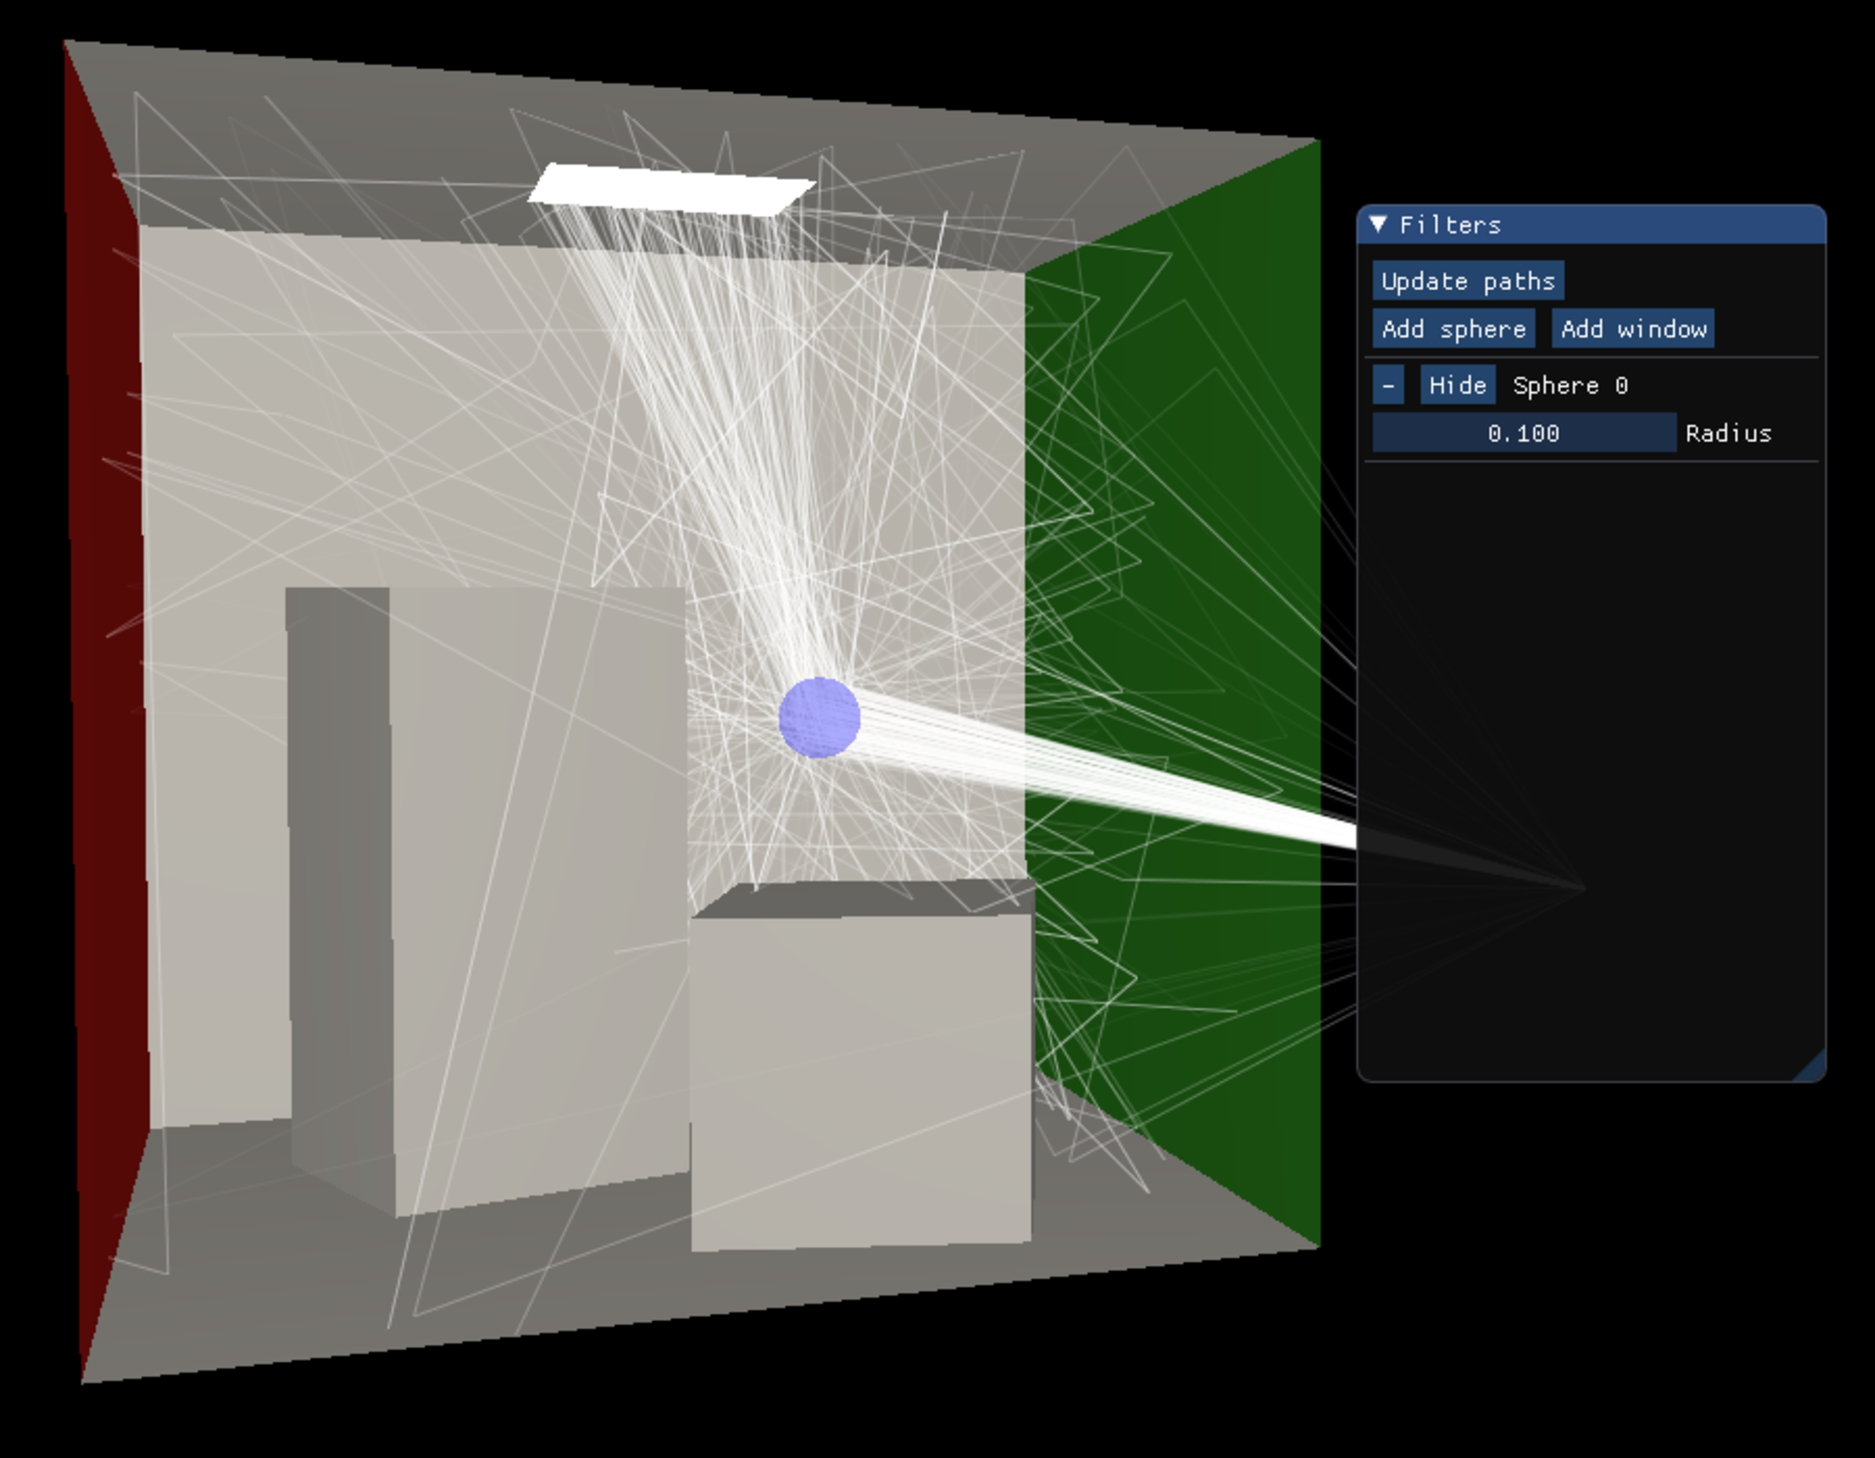
\includegraphics[width=\textwidth]{chapters/chapter_thetool/filterscombination1.pdf}
		\caption{In the beginning, one sphere is placed on the back wall.}
	\end{subfigure}
	\begin{subfigure}[t]{0.49\linewidth}
		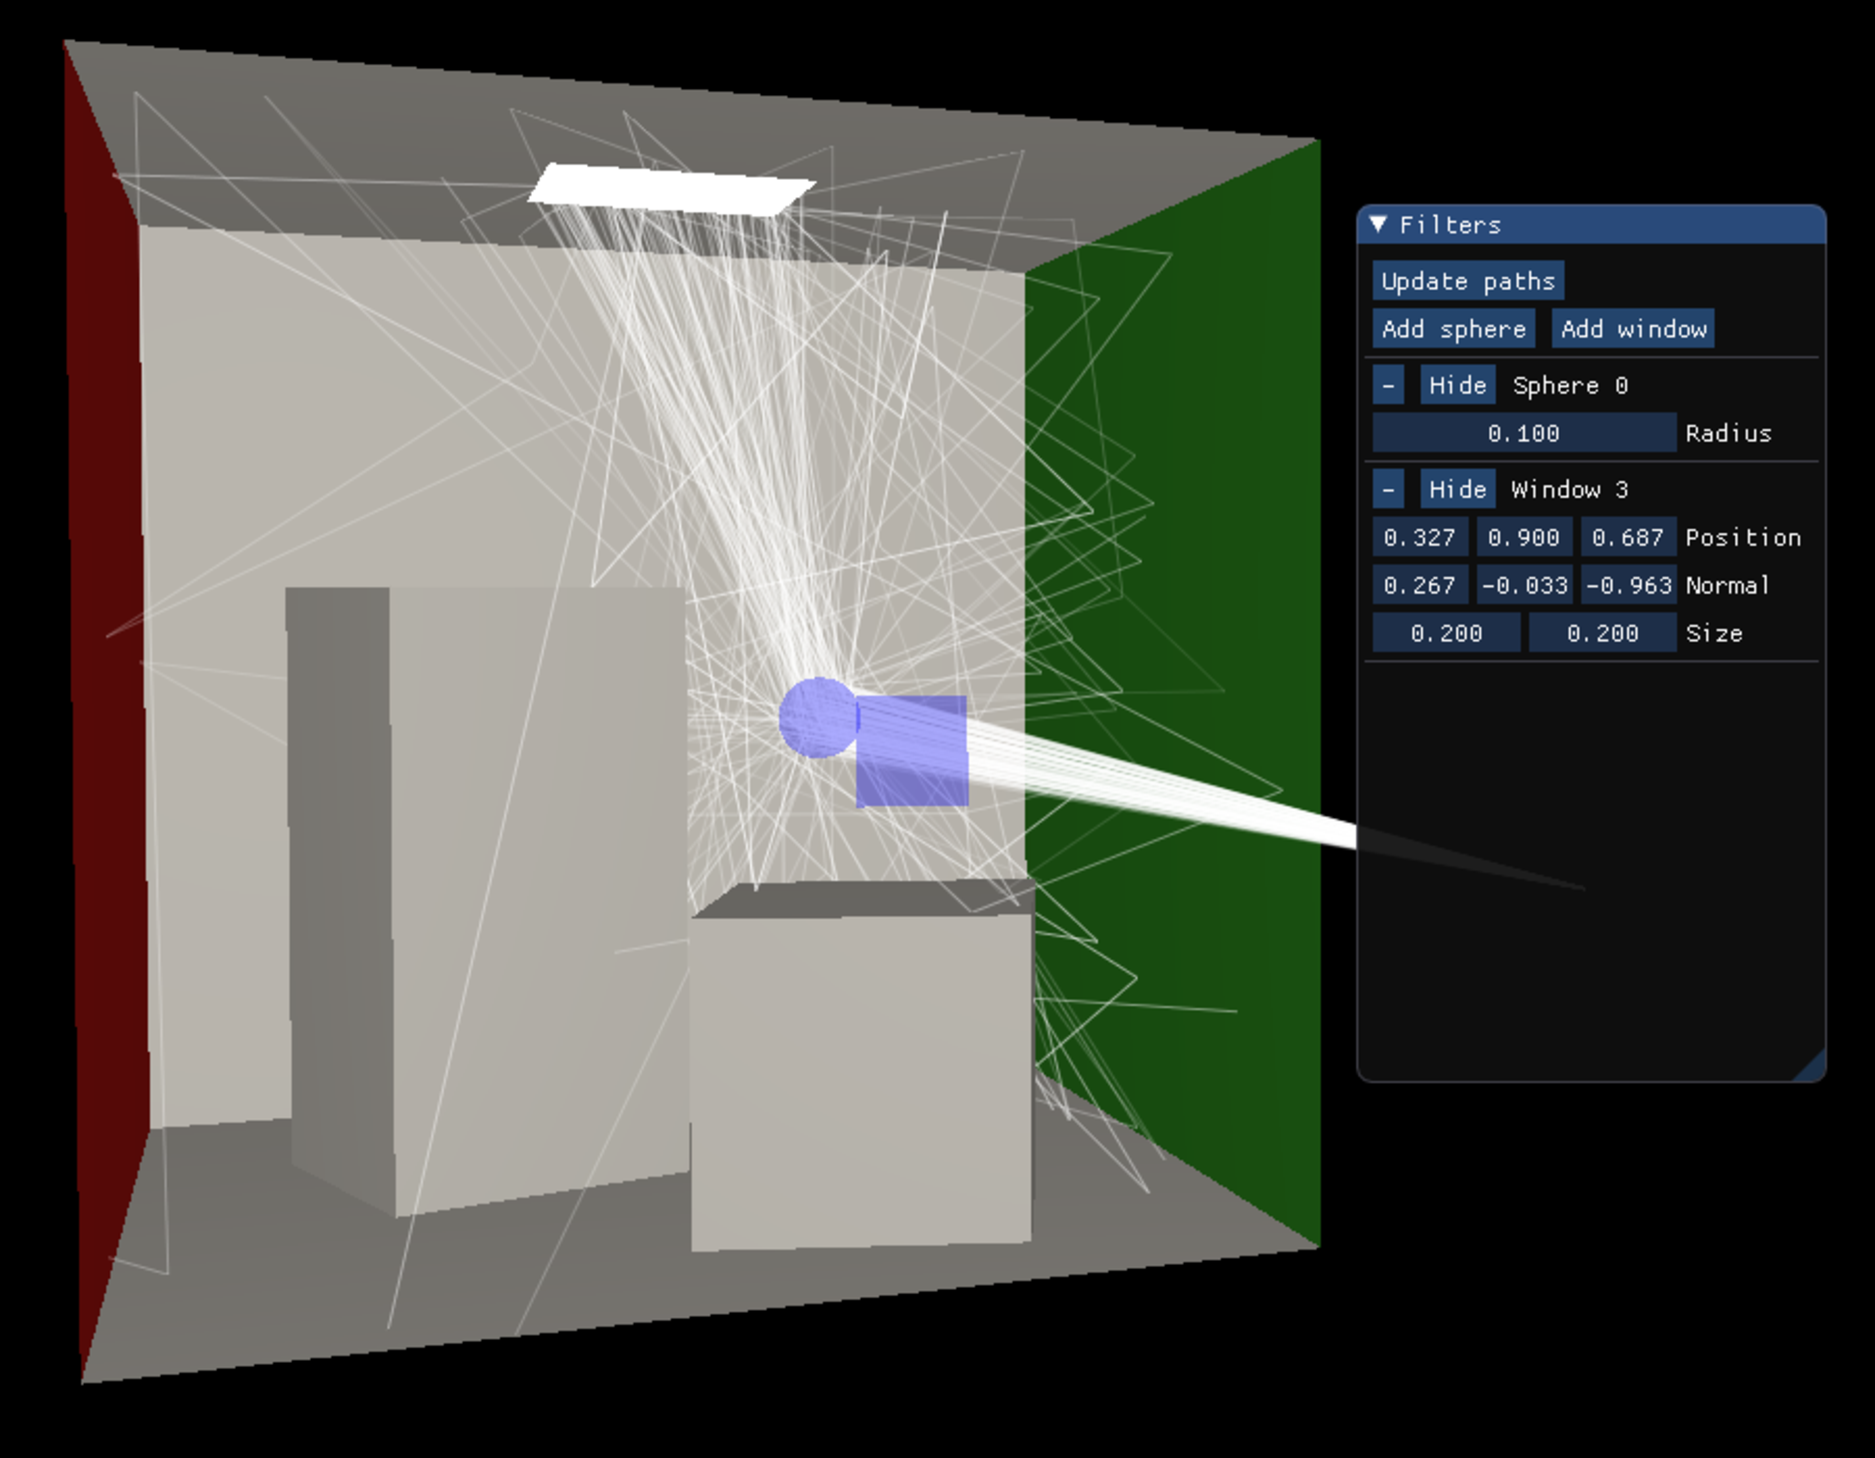
\includegraphics[width=\textwidth]{chapters/chapter_thetool/filterscombination2.pdf}
		\caption{Then a window is placed to select only the paths that go from the camera to the sphere on the back wall.}
	\end{subfigure}
	\begin{subfigure}[t]{0.49\linewidth}
		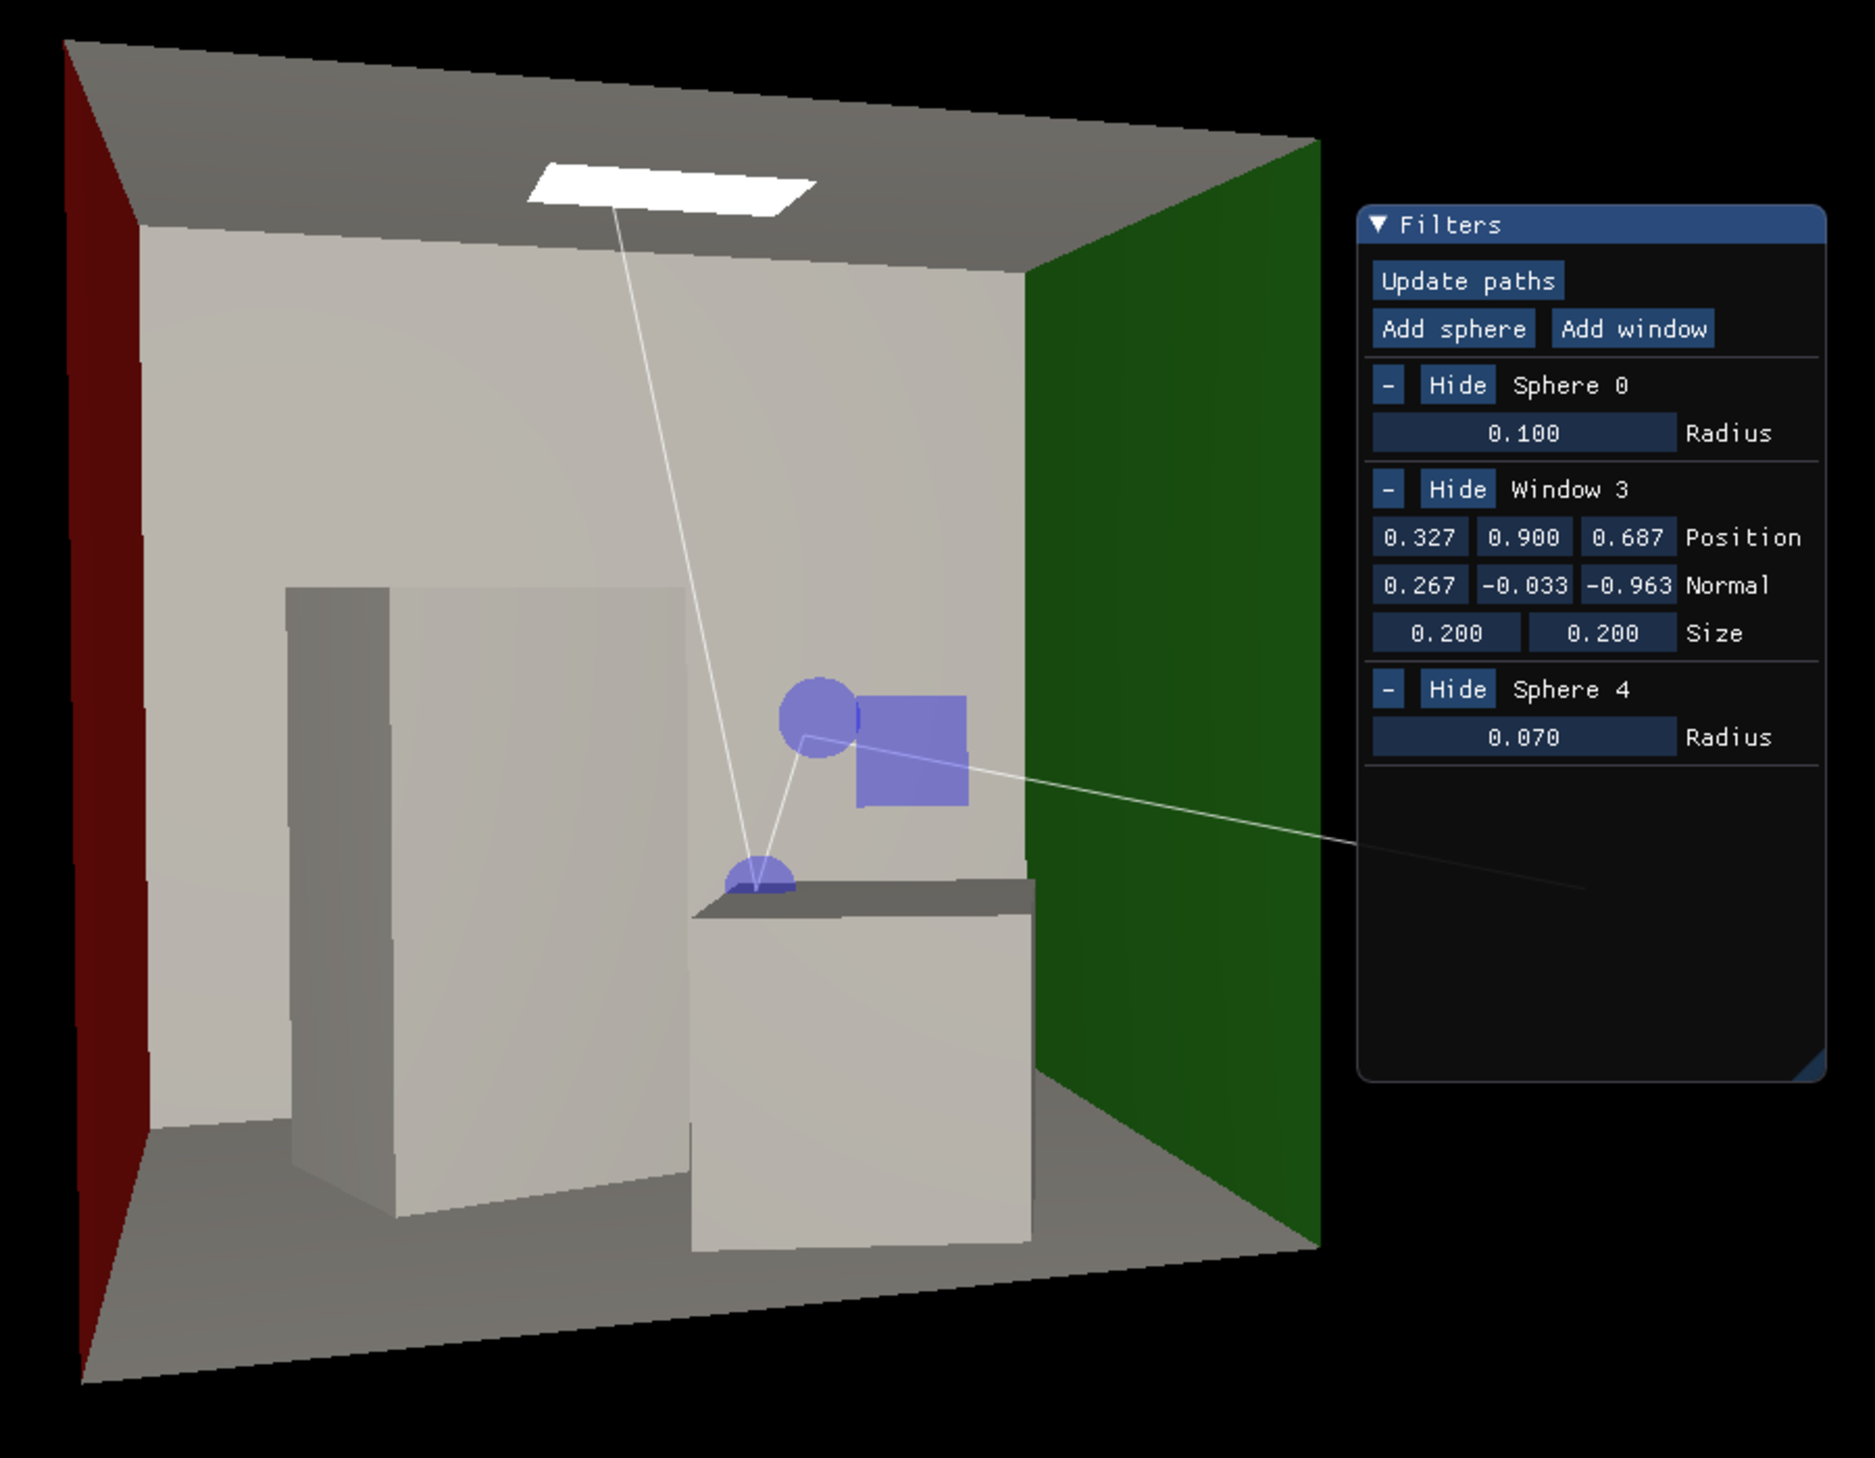
\includegraphics[width=\textwidth]{chapters/chapter_thetool/filterscombination3.pdf}
		\caption{Finally, a second sphere is placed on top of the short box to select only a single path.}
	\end{subfigure}

	\caption{Example of using more path filters together in a small dataset generated on the Cornell Box scene of $64 \times 64$ pixels and 32 spp.}
	\label{filterstack}
\end{figure}

Visualizing all paths at once is both useless and impossible in most cases. Useless due to visual clutter --- see figure \ref{visual_clutter} --- and impossible because most consumer grade GPUs cannot render several gigabytes of paths at once and keep an interactive frame rate.
User can filter paths so they can focus only on the scene portions they are interested in. Two filters types are provided: the \textit{sphere filter} and the \textit{window filter}. The former is a sphere that has to be placed on a scene surface and selects the paths bouncing inside its radius, the latter is a rectangular window that selects the paths passing through it.

As shown in figure \ref{filterstack}, combination of filters of both kinds can be used together. Considering all paths as a mathematical set of distinct paths $\mathcal{S}$, a filter $F$ creates a subset $F(\mathcal{S}) \subseteq \mathcal{S}$, and combining the filters $F_1, F_2, ..., F_n$ gives the intersection of their relative subsets:
\begin{equation}
	\label{filters_union}
	F_1(\mathcal{S}) \cap F_2(\mathcal{S}) \cap ... \cap F_n(\mathcal{S}) \subseteq \mathcal{S}
\end{equation}
Due to this strong affinity to mathematical sets, the initial code handling the filters' combination was mostly based on the \texttt{std::set<T>} data structure of C++ standard library. It was put apart when it turned out to be significantly slower than just storing everything into \texttt{std::vector<T>} structures and performing set intersections with the \texttt{std::set\_intersection} function from the \texttt{<algorithm>} STL library. To further speed the filtering up, the filters are computed in order so they all need to just test the paths selected by the previous filter; in the implementation, equation \ref{filters_union} is practically evaluated as if it was:
\begin{equation}
	F_n( ... F_2(F_1(\mathcal{S}))) \subseteq \mathcal{S}
\end{equation}
The tool uses a \texttt{std::vector<unsigned>} called \texttt{selectedpaths} to keep the indexes of the currently selected paths. Each filtering step is practically run over the \texttt{selectedpaths} output by the last stage. Before any filter, \texttt{selectedpaths} is filled with all path indexes. Forcing this into mathematical notation gives that the $i$th filter step out of $m$ filters is:
\begin{equation}
	\texttt{selectedpaths}_i = F_i(\texttt{selectedpaths}_{i-1}),\ i\in[1, m]
\end{equation}
where $\texttt{selectedpaths}_i$ is the \texttt{selectedpaths} vector after filtering through the $i$th filter and $\texttt{selectedpaths}_0 = \mathcal{S}$.

Users can add, modify and delete filters from the “Filters” floating panel. On the top of it there are three push buttons:
\begin{description}
	\item[“Update paths”] Since path filtering is an operation that takes a noticeable time to complete, the user must explicitly express the will to apply the current filter set to the paths.
	\item[“Add sphere”] After the user clicks this, they have to click on a surface of the scene. A filter sphere will appear on the clicked surface.
	\item[“Add window”] Same as the previous button but it adds a window filter on the clicked scene surface instead.
\end{description}
Filters currently present in the scene will appear right below these buttons. Each filter has an entry and all of these will have a delete button --- marked with a minus “-” sign ---, a “Hide”/“Show” button to toggle the filter visibility in the viewport, and a label with the filter name. Then, according to their filter type, there will be sliders controlling miscellaneous attributes.

\subsubsection{Sphere filter}

This was the first filter added. It has a spherical shape and simply selects all the paths having at least one bounce inside its volume. Users can place a sphere filter on clicking on any scene surface on the viewport after having clicked the “Add Sphere” button at the top of the “Filters” panel. Once a sphere filter has been added, its radius can be controlled by the slider in its slot on the panel. The default radius is one tenth of the scene largest dimension. One possible future improvement would be giving the possibility to translate the sphere after it has been initially created; might this be achieved through 3d gizmos or just by dragging, every step in that direction should help the usability.

The actual path filtering is plainly done by computing the squared distance between each bounce of each path and the sphere center. For each bounce with a computed distance less than the sphere radius, its entire path gets flagged as selected. This allows for a path-wise early termination: if a path has been flagged, it is useless to check the remaining bounces of the same path. Early termination or not, this computation is rather heavy since a render dataset rarely goes under the one hundred million bounces mark. To mitigate the otherwise lengthy waiting times, the computation is done on multiple threads; The set of paths that has to be filtered is divided in $n$ subsets $S_{1...n}$ of roughly the same cardinality, where $n$ is the number of maximum thread concurrency available on the machine. Each subset is coupled with a \texttt{std::vector<unsigned>} that has to hold the indexes of the paths of the subset that satisfy the filter; to avoid memory allocations, these vectors reserve $|S_{1...n}|$ slots each before any computation. Then, $n$ threads start to apply the filter to their assigned subset. Once all of them are done, the content of the vectors --- which are the indexes of the selected paths by each thread --- are moved into \texttt{selectedpaths}, the STL vector keeping the index of all selected paths.

\subsubsection{Window filter}



\subsection{Bounce density heatmap}
It might be extended by letting users draw transfer maps over a histogram.


\subsection{Viewport rendering}
\begin{itemize}
	\item Scene rendering
	\item Paths rendering
	\item Transparency 
	\item Camera control
\end{itemize}

\subsection{Scene format}
\label{scene_format}

As mentioned before, this tool uses an ad hoc scene description format. This format supports only triangle meshes and represents each with one vertex and one index buffer. A whole scene is contained in a JSON \cite{rfc8259} and a binary file. They must have the same name and respectively have the \texttt{.json} and \texttt{.bin} extension. 

The binary file contains all the mesh buffers as a contiguous sequence of little-endian 32bits numbers. While vertex buffers are stored as arrays of single precision floats, index buffers are arrays of unsigned integers. 

The JSON file beside containing information about the camera and the render image, it lists the scene geometries. For each it stores a color, a flag determining if the object is in any way translucent, a name, and buffer descriptions for both the vertex and the index buffer. These have a field holding their type --- which is either \texttt{vertices} or \texttt{indices} ---, an \texttt{offset} field determining the distance in bytes from the beginning of the binary file to the first byte of the buffer, and a \texttt{size} field storing the size of the buffer in bytes. For detailed information on the JSON structure a schema is provided in Appendix \ref{json_schema}.

\begin{figure}
	\centering
	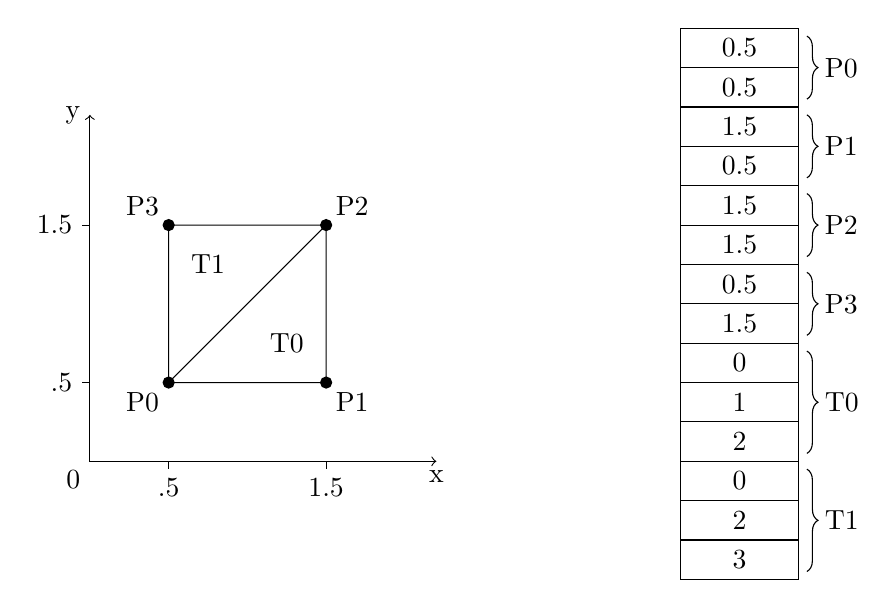
\begin{tikzpicture}
		% 2D scene
		\begin{scope}[shift={(0,0)}, scale=2]
			\draw[<->] (2.2,0) node[below]{x} -- (0,0) -- (0,2.2) node[left]{y};
			\draw (.5,0) -- (.5,-0.05) node[below]{.5};
			\draw (1.5,0) -- (1.5,-0.05) node[below]{1.5};
			\draw (0,.5) -- (-0.05,.5) node[left]{.5};
			\draw (0,1.5) -- (-0.05,1.5) node[left]{1.5};
			\begin{scope}[shift={(0.5,0.5)}]
				\draw (0,0) -- (0,1) -- (1,1) -- (0,0) -- (1,0) -- (1,1);
				\filldraw (0,0) circle (1pt) node[below left]{P0};
				\filldraw (1,0) circle (1pt) node[below right]{P1};
				\filldraw (1,1) circle (1pt) node[above right]{P2};
				\filldraw (0,1) circle (1pt) node[above left]{P3};
				\node at (.25, .75) {T1};
				\node at (.75, .25) {T0};
			\end{scope}
			\node[below left] at (0,0) {0};
		\end{scope}

		\begin{scope}[shift={(9,5.5)}, xscale=1.5, rotate=180]
			\draw (0,7) -- (0,0) -- (1,0) -- (1,7); 

			\draw (0,.5) -- (1,.5);
			\node at (.5, .25) {0.5};

			\draw (0,1) -- (1,1);
			\node at (.5, .75) {0.5};

			\draw (0,1.5) -- (1,1.5);
			\node at (.5, 1.25) {1.5};

			\draw (0,2) -- (1,2);
			\node at (.5, 1.75) {0.5};

			\draw (0,2.5) -- (1,2.5);
			\node at (.5, 2.25) {1.5};

			\draw (0,3) -- (1,3);
			\node at (.5, 2.75) {1.5};

			\draw (0,3.5) -- (1,3.5);
			\node at (.5, 3.25) {0.5};

			\draw (0,4) -- (1,4);
			\node at (.5, 3.75) {1.5};

			\draw (0,4.5) -- (1,4.5);
			\node at (.5, 4.25) {0};

			\draw (0,5) -- (1,5);
			\node at (.5, 4.75) {1};

			\draw (0,5.5) -- (1,5.5);
			\node at (.5, 5.25) {2};

			\draw (0,6) -- (1,6);
			\node at (.5, 5.75) {0};

			\draw (0,6.5) -- (1,6.5);
			\node at (.5, 6.25) {2};

			\draw (0,7) -- (1,7);
			\node at (.5, 6.75) {3};

			\draw [decorate,decoration={brace,amplitude=4pt},xshift=-2pt]
			(0,0.1) -- (0,0.9) node [right,midway,xshift=3pt]{P0};
			\draw [decorate,decoration={brace,amplitude=4pt},xshift=-2pt]
			(0,1.1) -- (0,1.9) node [right,midway,xshift=3pt]{P1};
			\draw [decorate,decoration={brace,amplitude=4pt},xshift=-2pt]
			(0,2.1) -- (0,2.9) node [right,midway,xshift=3pt]{P2};
			\draw [decorate,decoration={brace,amplitude=4pt},xshift=-2pt]
			(0,3.1) -- (0,3.9) node [right,midway,xshift=3pt]{P3};

			\draw [decorate,decoration={brace,amplitude=4pt},xshift=-2pt]
			(0,4.1) -- (0,5.4) node [right,midway,xshift=3pt]{T0};
			\draw [decorate,decoration={brace,amplitude=4pt},xshift=-2pt]
			(0,5.6) -- (0,6.9) node [right,midway,xshift=3pt]{T1};
		\end{scope}
	\end{tikzpicture}

	\caption{Geometry example. To simplify, a 2-dimensional case is presented. On the right a simple triangulated mesh is shown, on the left there is a valid binary file. A corresponding JSON file is shown in Listing \ref{scene_json}.}
	\label{scene_bin}
\end{figure}

\begin{Listing}
	\begin{lstlisting}
{
	"camera": {...},
	"render": {...},
	"geometries": [
		{
			"name":     "quad",
			"material": {...},
			"buffers": [
				{
					"offset": 0,
					"size":   32,
					"type":   "vertices"
				},
				{
				 	"offset": 32,
				 	"size":   24,
				 	"type":   "indices"
				}
			]
		}
	]
}
	\end{lstlisting}
	\caption{JSON scene file example relative to Figure \ref{scene_bin}. Information not relative to the geometry shape has been omitted. Please also remember this is a 2-dimensional example, hence the vertex buffer size is only 2 dimensions * 4 points * 4 bytes = 32 bytes instead of being 48 bytes like it would be in the ordinary 3-dimensional case.}
	\label{scene_json}
\end{Listing}

\printbibliography

All links were last followed on \today.

\appendix
\chapter{Scene format JSON schema}
\label{json_schema}

Is hereby presented a JSON schema\cite{handrews-json-schema-02} on which the JSON file of the scene description format must be built upon. Refer to Subsection \ref{scene_format} for more information on the scene description format. 
\begin{lstlisting}
{
	"type": "object",
	"properties": {
		"camera": {
			"type": "object",
			"description": "Camera properties"
			"properties": {
				"eye": {
					"type": "array",
					"description": "World position of camera eye"
					"minItems": 3,
					"maxItems": 3,
					"items": {
						"type": "number"
					}
				},
				"look": {
					"type": "array",
					"description":
						"World normalized vector of camera look direction"
					"minItems": 3,
					"maxItems": 3,
					"items": {
						"type": "number"
					}
				}
			}
		},
		"render": {
			"type": "object",
			"description": "Rendered image properties",
			"properties": {
				"width": {
					"type": "integer",
					"description": "Width (in pixels) of the rendered image"
				},
				"height": {
					"type": "integer",
					"description": "Width (in pixels) of the rendered image"
				},
				"spp": {
					"type": "integer",
					"description": "Samples Per Pixel of the rendered image"
				}
			}
		},
		"geometries":{
			"type": "array"
			"items": {
				"type": "object",
				"description": "A single geometry",
				"properties": {
					"name": {
						"type": "string"
					},
					"buffers": {
						"type": "array",
						"items": {
							"type": "object",
							"description": "Buffer description",
							"items" {
								"type": {
									"type": "string",
									"description": "Type of buffer",
									"enum": ["indices", "vertices"],
								},
								"offset": {
									"type": "integer",
									"description": 
										"Offset (in bytes) relative to the binary file"
								},
								"size": {
									"type": "integer",
									"description": "Size (in bytes)"
								}
							}
						}
					},
					"material": {
						"type": "object",
						"description": "Basic material description",
						"items" {
							"color": {
								"type": "array",
								"minItems": 3,
								"maxItems": 3,
								"items": {
									"type": "number"
								}
							}
							"translucent": {
								"type": "boolean"
							}
						}
					}
				}
			}
		}
	}
}
\end{lstlisting}

\pagestyle{empty}
\renewcommand*{\chapterpagestyle}{empty}
\Versicherung
\end{document}
